\chapter{Implementation \& Testing}
Following from the analysis and design of the application, it is now possible to start implementing the features produced from investigating the requirements earlier in the project. As it was already stated that the project would be running under an FDD means, rather than having two sections (one for implementation and one for testing), this section will show each feature one-by-one. By following this scheme, the feature prioirty list will be utalised to ensure the more important features are done first, and that they fulfil their function before moving on. However, this should not hide the fact that issues are possible when implementing and any such issues could hamper further development. If this does occur, the issues and reasons will be explained, followed by what judgement was made to continue on with development of the application as a whole.

\section{FDD project approach}
As mentioned, the feature driven development methodolodgy will now shape the approach that is taken to create each feature. Although design has already been completed for all features, there are still elements to each iteration that should be outlined before proceeding. The best way to plan this is to give a brief list of steps that will be performed in each iteration. This is as follows:

\begin{enumerate}
\item Give a re-cap on the requirements of the feature
\item Provide a walkthrough of implementation (with code samples)
\item Show tests used (JSUnit, usability tests) and results
\item Describe and differences with the feature and original design
\item If there are any issues, describe and give explanations
\item Give a progress log on the item, and provide dates and length of completion for use in accordance with the Gantt chart originally constructed
\end{enumerate}

It should also be noted that once the duration of the time in the project for the implemtation and testing stage is complete, a burn down and progress report will be possible to generate and will be done so. This will give a good idea of exactly the status of the project (with a calculated percentage), to see how much work was done compared to estimates, and to find out how succesful the project was overall. 

\subsection{Iterative Implimentation}
Before the iterations begin, it should be mentioned that although the order of features to be implemented were decided in the analysis, in order to impliment any back end things and allow for proper testing (usability testing), some basic GUI must be created first. Becuase of this, this will be the first iteration, followed by creation of the JSON manoeuvres. Following these iterations, it will then be much easier to test future features created. Without a basic GUI and canvas, it will be impossible to see the effects created whilst adding features such as drawing flight paths or moving cameras. After these two moved features are complete, the prioritised list will run as planned initially.

\subsubsection{Feature 1- Create a basic GUI}
The first feature that was to be implemented was less of a feature but more a requirement so the other features could be then created. The GUI or front-end of the application is important to be created, otherwise testing future WebGL features will not be possible. The requirements of the front end were:

\begin{itemize}
\item A responsive front-end that is mobile compatible
\item Have hidden menus that can push in from the left
\item Have basic inputs such as the OLAN input, and menu options
\item Provide a help and about page that overlays the application web page
\end{itemize}

The first task that was performed to create this task was to create a minimulistic layout matching the wireframes designed in chapter 2 of this report. The first action performed was to get the latest Foundation \cite{foundation} css library file, and then to create a layout using the features from the library. The navigation was made using the 'navbar' markup, which helps stick the navbar to the top of the page, alongside automatically changing into a mobile pull down menu once the screen size reaches a certain amount. Then using other mark-ups provided by Foundation I was able to float the various navigation bar buttons to their respective sides. 

The most important part of the GUI which has now been implimented is the off-canvas feature menus. The code for this can be seen in section~\ref{code:canvas} of appendix C. The way that Foundation helps create this off cnvas option is by wrapping everything in one div, then seperating the menu and content in half. When a user then pushes the designated button with the wrapper id, the entirety of the wrapper is pushed to the right to display the menu and less of the content. The about and help pages were also added successfully, with the addition of another library called Modernizer. This library allowed for a clean effect to overlay the information on top of the webpage.

Once the basic HTML elements with relevent ID tags were added to the index page of the application, it was then possible to add some custom style to the page. As mentioned in the design stage, it was possible to download Foundation modified with the colour scheme designed for the application. Changing backgrounds to black and text to white was very easy, and then added to the site. The colour and design of the page can be seen below in figure~\ref{fig:newgui}.

\begin{figure}[h]
  \centering
      %\includegraphics[width=1\textwidth]{images/newgui.png}
  \caption{Screenshot of GUI created with Foundation, JQyery and HTML markup.}
  \label{fig:mod}
\end{figure}

As planned, Sass was used to style specific elements of the page, such as the width of the OLAN input box, and to change text placement on the help and about pages. Setting up the Sass with Koala was easy, and upon each save of the file, CSS was compiled. 

One final mention goes to the creation of the WebGL canvas. To create the basic canvas, only a few lines of JavaScript was needed. To create it, a renderer was created using  the 'THREE.WebGLRenderer' object. Becuase this is early in the implementation stage, it was created without RequireJS as the archetcure is only one JS file. Once the object is created, JQuery appends the '.domElement' of this object to the container div created in the basic HTML. For future features, the WebGLRenderer object with be where any objects such as flight paths are added to.

As for testing this feature, becuase very little JavaScript was required to be coded here, usability testing was the only way to check for the completion of what was required. The test results can be found in Appendix D under section~\ref{test:canvas}. Overall, this feature has been made to 100\% of the requirements laid out, and matches the deisgn very well. Therefore, the progress tracker for this feature can be shown as:

\begin{table}[h]
\begin{tabular}{|l|l|l|l|p{7cm}|}
\hline
\textbf{Start} & \textbf{End} & \textbf{Duration} & \textbf{Progress} & \textbf{Comments}                                                                                                     \\ \hline
09-03-2015     & 10-03-2015   & 2 Days            & 100\%             & Complete, though once new features are under way, RequireJS will be utalised and the WebGL Canvas code will be moved. \\ \hline
11-03-2015     & 11-03-2015   & 1 Day            & 100\%             & Testing complete, usability table created and tested on mobile and desktop devices.\\ \hline
\end{tabular}
\end{table}

\textbf{Feature overall progress: 100\%}

\subsubsection{Feature 2- Convert OLAN and Aresti to JSON form}
The second feature, which was of high importance to the rest of the application was to create OLAN interpreted JSON which would give instrctions on how to construct each manoeuvre. Becuase this was quite thoughroughly planned and then designed how each instruction was going to broken down, the time designated for this task felt generous. Simply using the template created in the design, it was possible to fill in each instrction part by part through each OLAN manoeuvre. An example of some instructions can be seen in Appendix C in section~\ref{code:jsonmoves}.

The only time consuming part of this feature was the shear amount of different manoeuvres that had to be converted. For this reason, not every OLAN letter was created. The reason for this is becuase some moves are possible to be created from others, so further in development, more will be possible to be added. 

To support this feature, more JavaScript code had to be added to allow the JSON to be read into an object to begin drawing moves onto the canvas. Becuase the code would be in a different module to the WebGL canvas that was created in the previous feature, RequireJS now had to be added to the source code. To do this, the RequireJS library was added and initiated in the HTML page of the application as shown here in Appendix C section~\ref{code:requireJS}. Then a new module was created, named 'Dataparser' as designated in the design. The method for converting the JSON can also be found in the data parser module shown again in the appendix under section~\ref{code:jsonmovesJS}.

Once the coding and converting to JSON was complete, testing the code that performed the conversion to an object was required. By using JSUnit, it was possible to call the method that was created to instantiate the manoeuvres array, and pass in some raw JSON string, then compare to what the result should be. The JSUnit code can be found in appendix D, section~\ref{test:jsonmvoes}.

Like the last feature, no changes from the original design were performed, resulting in a good standing of time compared to the Gantt chart for the project. The feature progress can be expressed as percentages and final comments added again.

\begin{table}[h]
\begin{tabular}{|l|l|l|l|p{7cm}|}
\hline
\textbf{Start} & \textbf{End} & \textbf{Duration} & \textbf{Progress} & \textbf{Comments}                                                                                                     \\ \hline
12-03-2015     & 16-03-2015   & 5 Days            & 80\%             & JSON created to represent most manoeuvres, for that reason it is not an exact 100\& progress. JavaScript code and RequirejS functionality added to support the rest of the application. \\ \hline
17-03-2015     & 18-03-2015   & 2 Days            & 100\%             & JSUnit tests created and passed successfully, showing JSON matches up with manouvre array object.\\ \hline
\end{tabular}
\end{table}

\textbf{Feature overall progress: 90\%}

\subsubsection{Feature 3- Creating a scene with terrain and lighting}
The third feature, which is another to be brought forward ahead of flight path creation is the terrain and lighting effects. The reason for creating this before the OLAN construction is the same as creating the canvas, becuase without an area to see where the paths are drawn onto, the effects of that feature will be hard to test if it is working. Especially terrain, where the need for this is to see where the X axis of 0 will be. Without this, when implementing checks such as if the path would hit the ground would be harder to test. Again, the three.js library was of great use here, especially with built in methods to allow for lighting to be added.

In order to have started this feature, another module was added to the archetecture named 'TerrainHandler', which was where both lighting and ground was to then have their methods of adding to the canvas. This feature was found to be the shortest of the features, as it only required two simple methods. Rather than passing the renderer canvas object to this module to add the ground and lighting, it was decided to simply make both methods like factories to return the ground and lighting objects to where they were called from. In the case of where this module was called from, the main class where the canvas was created seemed the best place to call each method, as everything to do with setting up the scene could remain together and be easily understood or developed further.

As for testing, by keeping the terrain and lighting in their own module also helped towards testing the new methods. Two very simple tests were made using JSUnit to check the returns of each method, and both were added to the Jasmine instructions under each Github commit through the Travis builds. As with other tests, the test cases can be found in the appendices under appendix D section~\ref{test:lights}. This feature was fairly straight forward to implement and test with help from the three.js documentation site, therefore teh feature was done in less time than originally planned.

\begin{table}[h]
\begin{tabular}{|l|l|l|l|p{7cm}|}
\hline
\textbf{Start} & \textbf{End} & \textbf{Duration} & \textbf{Progress} & \textbf{Comments}                                                                                                     \\ \hline
19-03-2015     & 20-03-2015   & 1 Day            & 100\%             &  Completed module for terrain and lighting, linked up to main module.\\ \hline
20-03-2015     & 20-03-2015   & 1 Day            & 100\%             &  Two JSUnit tests created, and passing successfully.\\ \hline
\end{tabular}
\end{table}

\textbf{Feature overall progress: 100\%}

\subsubsection{Feature 4- Cameras}
The final predessing feature before the creation of OLAN paths that was decided should be ready were the various cameras that will look around the canvas. The initial requirements for cameras was to have two different views: one for navigating around the canvas, and the other for being onboard the flight path. At this stage of the project, creating the second was only possible to a certain extent, becuase without the construction of the paths yet, getting the location of where the onboard camera should be is not possible. Therefore, for this requirement both cameras were created, with the exception of the onboard camera where functionality is currently restricted. 

To start, another module was created for the 'CameraController'. Becuase it was best to keep the cameras completely seperated from other parts of the application to reduce decoupling, both camera objects were stored in this module and provided get and set methods for calls from other modules. An inititiator method was created for use from the main module, to create both camera objects at start up. Both these objects were again availible from the three.js library as 'THREE.PerspectiveCamera'. Then by passing the module around to any other modules, it will then be possible to update and retreive each camera object again. Alongside the camera creation, a controller for changing the angle of view, zoom and co-ordiantes was created as another module. 

This module, which has been called 'CanvasController' as designed in the module diagram, adds event listeners for dragging the mouse around the canvas, keyboard presses to move up and down, and scroll for zooming. Then by getting the new updated values of view-point angles, these are passed back to the camera controller which updates the values of each camera. By repeating this in a render loop in the main module, the updating of cameras is done several times a second, to make movements appear fluid. To help this, the code was refeactored several times to ensure that the amount of work done by the browser is as little as possible on each loop of the animation.

As for testing, alike the first feature where usability testing was the primary and sole means of checking the implementation fulfills the feature, JSUnit testing was not used. Usability testing was found the best option here, and results can be found in appendix D section~\ref{test:cameras}. During testing, it was found that there was an issue that when rotating the camera around the canvas, it seemed to always rotate around the point (0,0,0). This meant that navigating the canvas was slightly harder than it should have been. This was fixed though, by simply moving the camera rather than the scene in the canvas. As for the camera that was designed to be as on board view, a model airplane was added to represent the camera so it could be seen on the canvas. Although it does not move yet, the plane loads up at the start of the application and can be placed anywhere on the scene. You can see the plan on the canvas at point (0,0,0) below in figure~\ref{fig:plane}. The plane model is constrcuted from a JSON file from a page on the web with thousands of free models.

\clearpage

\begin{figure}[h!]
  \centering
      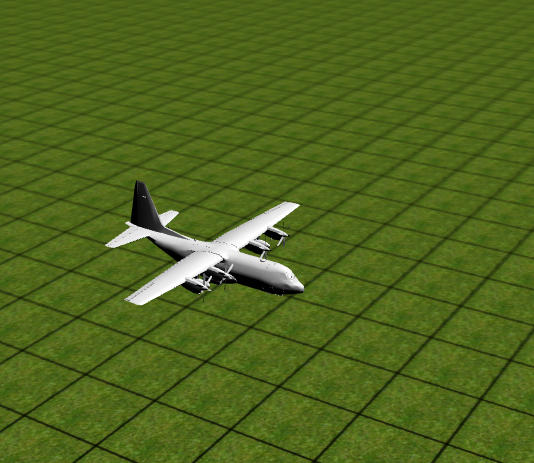
\includegraphics[width=0.6\textwidth]{images/plane.png}
  \caption{Model of plane loaded up using JSON and three.js object loader. This plane will represent the onboard camera, and fill be the object that will be assigned locations along an OLAN path to show flying the flight plans entered by users.}
  \label{fig:plane}
\end{figure}

The progress of the task is shown below. This feature was done exactly to its requirements in the design, and the modulation of code is still being followed.

\begin{table}[h]
\begin{tabular}{|l|l|l|l|p{7cm}|}
\hline
\textbf{Start} & \textbf{End} & \textbf{Duration} & \textbf{Progress} & \textbf{Comments}                                                                                                     \\ \hline
21-03-2015     & 23-03-2015   & 3 Days            & 100\%             &  Both cameras now usable, with constructer methods, and update methods. On board camera ready but not linkable to rest of application until animation of flight paths is ready.\\ \hline
24-03-2015     & 24-03-2015   & 1 Day            & 100\%             &  Usability tests complete, one change made to code following a failed test. \\ \hline
\end{tabular}
\end{table}

\textbf{Feature overall progress: 100\%}

\subsubsection{Feature 5- Construction of 3D paths from OLAN}
The most important feature, drawing shapes onto the canvas using the instrctions read in from JSON files was next to be implemented. The main requirement here was to draw smooth shapes that match the Aresti shapes as accuratly as possible, also bearing in mind that they should be linkable.

Using the array of maneouvre objects inported from JSON in the first feature implemented, creating shapes based on these was a matter of building up an array of vectors with each new vector being copied from the previous and then having the next instruction take effect on it. To do this, under a new module 'ManouevreController', a method was created that firstly found whih manouvre was to be built, then loop through the instructions of that manouevre creating it vector-by-vector. An example of how vectors were calculated is shown below in figure~\ref{fig:vectors}.

\begin{figure}[h]
  \centering
      %\includegraphics[width=1\textwidth]{images/vectors.png}
  \caption{Flow chart of how vectors were used to construct the spline shape.}
  \label{fig:vectors}
\end{figure}

As you can see, once vectors were created, they were passed to a three.js object which was a spline curve. A spline curve is one that interpolates along all its points to create a smooth shape. Once points are added to this object, it can then be added to the canvas. Upon initial usability testing of this, it was found that many of the joins between points were well-off center, due to the interpolation being too large. This was down to the fact that with each turn instruction being a 45 degree angle, meant that the change was too sharp from a straight to curved line, so the straight line was affected too much. To fix this, by dividing up the 45 degree into smaller pieces meant that interpolation was needed much less, therefore the curves appeared smoother and had much less effect on any predecessing straight lines.

Another big issue that appeared during testing was that any manoeuvres that had a change in angle through a turn always seemed to revert back to a straight line, meaning the rest of the manoeuvre was out of sync and did not look correct. This was an especially time-consuming bug, and a example of it can be seen in figure~\ref{fig:issue}. Becuase finding out the problem and attempting to fix it was eating away at other feature time, the issue was left for the time being, in order to complete other key features outlined in the requirments. In order to ensure this issue would not remain at the end of the project, a strict time limit was set on the next features to allow for a good amount of time to fix the issue here.

\begin{figure}[h]
  \centering
      %\includegraphics[width=1\textwidth]{images/vectors.png}
  \caption{Flow chart of how vectors were used to construct the spline shape.}
  \label{fig:vectors}
\end{figure}

At the end of the iterations in this report, this issue will be re-evaluated once the fix is in place. Other than this issue, the rest of the feature was implemented well, and entering OLAN now drew fairly accurate shapes. Again with testing, usability was the primary case here, becuase checking for correct spline curves created would be too time consuming and difficult with the use of JSUnit. The overall progress of the task at this point of the project is as follows:

\begin{table}[h]
\begin{tabular}{|l|l|l|l|p{7cm}|}
\hline
\textbf{Start} & \textbf{End} & \textbf{Duration} & \textbf{Progress} & \textbf{Comments}                                                                                                     \\ \hline
25-03-2015     & 05-04-2015   & 2 Weeks            & 75\%             &  Although OLAN now is represnted by shapes and they link up correctly, the issue mentioned os straight lines being drawn on change of angle remains. This will be fixed fully after implementtaion of other tasks.\\ \hline
06-03-2015     & 08-03-2015   & 2 Days            & 75\%             &  Usability tests complete, changed step of angles from 45 to 15 to get smoother interpolation. More tests will be required after fixing the issue.\\ \hline
\end{tabular}
\end{table}

\textbf{Feature overall progress: 75\%}

\subsubsection{Feature 6- Animate OLAN flight path}
Although there was an issue imnplementing the drawing of flight paths in the previous feature, the functionality that was complete allowed for the animation feature to be done. Three.js provided a good means of getting points along the spline curves to a percentage of the length of the shape. For example, by using the method 'getPointAt' with 50 as the paramter value gave the return vector value of the point on the line halfway. By doing this iterativly using the render loop used in the cameras meant a value could be incremented over time, thus getting points along each curve. Each time a point was received, the on-board camera could then be set to the position of it, and by doing this as fast as the render loop meant that a smooth animation was created. Again, a new module was created 'AnimationController' with various methods for playing and pausing the animation, and setting the distance of time between each point recieved in order to speed up or slow down the animation.

With each curve being stored in an array object, meant if linked up manoeuvres were being animated along, once one manoeuvre had reach 100\% for getting points along its line, the next manoeuvre would be selected from the array and the get-point percentage reset back to 0. By doing this, a flawless smooth cross between manoeuvres has been achieved.

As for testing this feature, more JSUnit was used, but mainly for the getters and setters of the controller. For instance, checking that the pause, play and speed setters worked correctly required simple test cases that checked the private variables holding the values were correct. Alongside these tests, usability tests were also completed becuase of the new buttons in the GUI representing the play/pause and speed options. Both tests can be found in the appendices under section~\ref{test:animation}. Following the completion of this feature, the progress can be reported on. 

\begin{table}[h]
\begin{tabular}{|l|l|l|l|p{7cm}|}
\hline
\textbf{Start} & \textbf{End} & \textbf{Duration} & \textbf{Progress} & \textbf{Comments}                                                                                                     \\ \hline
09-04-2015     & 10-04-2015   & 2 Days            & 100\%             &  Animation is now possible through all manoeuvres in a flight, alongside options to pause, play and change speed.\\ \hline
11-04-2015     & 11-04-2015   & 1 Day            & 100\%             &  Simple JSUnit and usability tests performed to check values from GUI are being sent to the back-end correctly.\\ \hline
\end{tabular}
\end{table}

\textbf{Feature overall progress: 100\%}

\subsubsection{Feature 7- Exporting and importing routines}
The last of the primary features planned for the applicatoin was the saving and loading of flight plans. Because up to this stage the project time was behind, and time was required to fix other issues, it was decided that the initial format of saving the OLAN input directly would be quicker top implement than the rendered vector values. 

To start this, a final module was created for the handling of JSON files and local storage, adn this was then linked up to the HTML handler module to get the user's current OLAN input value. Four methods were required for this:
\begin{enumerate}
	\item Exporting to JSON- This method makes a simple JSON file with one object contained ("OLAN" : olan string)
	\item Importing from JSON- Allowing selection of a user file from the browser, and selecting the OLAN from it, then entering this into the input box to be rendered.
	\item Exporting to local storage- The same format as the JSON, but saving in the browser. See appendix C section~\ref{code:localstorage}.
	\item Importing from local storage- same, should be automatic when application loads up
\end{enumerate}

In addition to the requirements that were implemented, it was decided that user should be able to choose whether automatic backup of the entered OLAN would load up at the start of the application. Becuase of the observer pattern that is being used throughout implementation, it took a very short space of time to add this feature to the HTML handler listener.

Testing involved some JSUnit again, where test data was entered and checked against the reuslting JSON and local storage objects. The tests can be seen in appendix D section~\ref{test:save}. Up to this point and for future tests, it was ensured that the Travis builds were passing when running all the JSUnit tests through Jasmine. This feature was completed quicker than the allocated time due to the research into Local storage previously, and therfore helped gain back some valuable time for other features.

As for any future development, it was mentioned that it could have been better to export the vectors directly, but the space in files and in time was considerable here therefore helping towards effiency in this part of the project. The ending progress of this feature follows in the table below.

\begin{table}[h]
\begin{tabular}{|l|l|l|l|p{7cm}|}
\hline
\textbf{Start} & \textbf{End} & \textbf{Duration} & \textbf{Progress} & \textbf{Comments}                                                                                                     \\ \hline
12-04-2015     & 14-04-2015   & 3 Days            & 100\%             &  Both importing and exporting of JSON and local storage complete, with an additional feature of giving the user the option to auto save when they enter any OLAN.\\ \hline
14-04-2015     & 15-04-2015   & 2 Days            & 100\%             &  Implemented JSUnit tests linked to the Travis build, testing the format and content of exported flight plans.\\ \hline
\end{tabular}
\end{table}

\textbf{Feature overall progress: 100\%}

\subsubsection{Feature 8- Adding further GUI options}
By this point, quite a few of the features installed into the application had the possibility of allowing the user to interact with a range of different paramters and options. For example, with the spline curves, there was options such as the smoothness of interpolation (the number of extrusion segments), options to switch between cameras, and the scale of flight paths amongst others. As with other options that had been added along the way with some features such as speed and auto-save, linking each to the GUI was fairly straight foward, with all that being required was to create an ID for the HTML element to be an option, and then listen for a change or click using the HTML handler, finally calling its respected method.  

The options that were added can be shown in a comprehensive list with reasonings for each.
\begin{itemize}
	\item Extrusion segments- The smoothness of paths, where the more the user chooses the more segments each curve is made of. This can help users with less powerful systems, as there is less to render with less segments.
	\item Onboard view- an option that changes the current camera view to one where the user will view the canvas enviromnent from the point of the view of the front of the aircraft. This gives the feel of actualyl flying the OLAN path, which could be helpful to users such as pilots who may want to learn a routine from the inside of a cockpit.
	\item Scale- The scale of all the OLAN paths drawn, defaulted at 1, but can be increased in multiples. Useful if the user wants to fit more onto the canvas, or wants to get a larger better view of a move.
	\item Radius segments- The initial line that is drawn to show the manouevre may be changed to have more sides. For example, the default being 2 means a flat ribbon is drawn. 1 would be a single line, whilst 0 would make the path invisible. This would then allow the user to have an aircraft fly the path without any shapes behind it.
\end{itemize}

An addtional GUI feature that was added here was the check for the loading of the OLAN JSON file before activating the input box in the navigation bar. As mentioned in design, this box shuold not be editable until the application is fully loaded, so a method was created in the HTML handler to activate the box when needed. This method was called by the camera controller module once the model aircraft was loaded, as this was the last and largest file to load.

As with any GUI interface features, usablity testing was the best option here, and therefore each new option added was tested after being created. The tests checked if the proper function was called and had an effect on the application as was planned. The tests follow the previous ones in appendix D under section~\ref{test:options}. It should be noted that the tests were done both on mobile and on desktop, to keep up with the added requirement that the application should be usable on both platforms. The tests ensured that all the options worked well, and worked when they were supposed to. The following table shows this feature's progess.

\begin{table}[h]
\begin{tabular}{|l|l|l|l|p{7cm}|}
\hline
\textbf{Start} & \textbf{End} & \textbf{Duration} & \textbf{Progress} & \textbf{Comments}                                                                                                     \\ \hline
15-04-2015     & 15-04-2015   & 1 Day            & 100\%             &  Options added to reflect changes in various aspects of the application, alongside the lazy initialisation check added to the OLAN input box.\\ \hline
16-04-2015     & 16-04-2015   & 1 Day            & 100\%             &  Usability tests performed on desktop and mobile browsers, all passing after multiple times refactoring. \\ \hline
\end{tabular}
\end{table}

\textbf{Feature overall progress: 100\%}

\subsubsection{Feature 9- Flight 'movie reel'}
The movie reel feature was one that would be added if there was enough remaining time, though in this case it was decided that it would be implemented to a set time limit. The aim of the reel would be to show the user what manoeuvre is currently being flown in the animation, by having images or teh manoeuvre from the OLAN input box converted to simple 2D Aresti, and then shown along a reel with current progress across them in relation to the entire flight. To start this, it was firstly considered that using the logic from the manoeuvre controller that built flight paths could be used to the same effect for drawing the movie reel figures. 

Upon starting this though, it was foudn that many aspects of the feature would take too much time to implement, and that they could cause performance issues for the user. The first of these was that if the application was going to draw mini figures at the bottom of the page in a fixed location, it would mean having to create a set of mini-canvases to interact with, rather than using the main canvas and drawing at the bottom of it. Each figure would thus need its own canvas, and after so many are added, this can dramatically affect the browser's perormance. Another issue foudn when looking how to create the reel was the complex style of Aresti figures required. For example, creating arrows to represent rolls, and for annotations to be generated in the correct places alongside curves would require detailed mechanics in the back-end in order to produce them. This and the first issue was decided would take up too much development time, thus pushing back the remaining features left to fix and implement. Therefore a compromise was made, where the reel has a range of images of the Aresti figures loaded and put in place alonside each other. These images have already been created using the OpenAero application, so saving these to a folder in the application was easy, and each was saved with the name of the OLAN letter. 

The movie reel was incorparated into the HTML handler, as this was a dom-element related item and required JQuery to manipulate the space at the bottom of the canvas. Then, added to the listeners in the HTML handler file was an event where when the user enters an OLAN letter, and this is found in the manoeuvres array (to ensure it is a real OLAN notation), an image representing the Aresti figure with the letter for the filename was loaded into a div floated at the bottom of the page where it was appended. Although this means of creating the figure was not what was initially planned, due to time constraints this means of creating the feature ensured it was done as quickyl as possible, but also to a good standard of presentation that fit well with the rest of the application. It can be seen in figure~\ref{fig:movie} the reel with some figures loaded up, with the current animation progress highlighted over the manouevres.

\begin{figure}[h]
  \centering
      %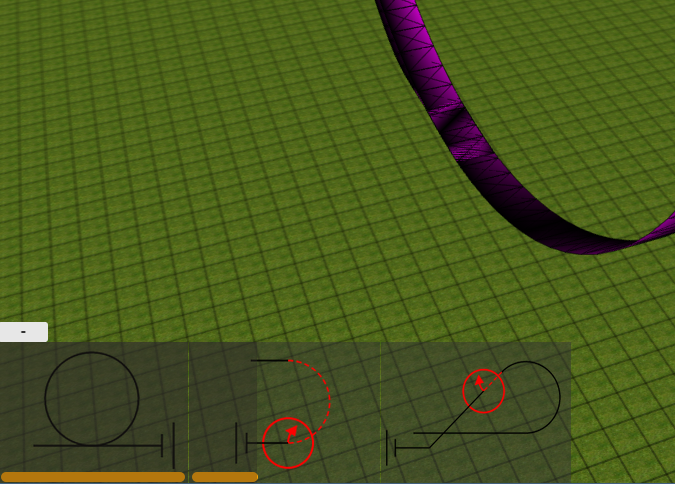
\includegraphics[width=1\textwidth]{images/movie.png}
  \caption{Movie reel overlaying the bottom of the canvas, with some figures loaded after the user typed in a string of OLAN.}
  \label{fig:vectors}
\end{figure}

Figure~\ref{fig:movie} also shows the animation progress, which was achieved by simply getting the current value of time which was used earlier in the 'getPointAt' method, then getting the percentage of this for the amount of moves entered. After this, a simple div was placed again using Jquery over the width of that percentage to achieve a darker coloured semi-transparent status bar. During tests of this feature (usability), one such issue was found that was caused when more than five manoeuvres were entered, the remaining Aresti figures were not present on the page, as it had been split into five sections. This means at this point of the project only the first five manoeuvres have their animation status shown. This is another feature that is hoped to be fixed before the end of the project implementation stage. 

\begin{table}[h]
\begin{tabular}{|l|l|l|l|p{7cm}|}
\hline
\textbf{Start} & \textbf{End} & \textbf{Duration} & \textbf{Progress} & \textbf{Comments}                                                                                                     \\ \hline
17-04-2015     & 19-04-2015   & 3 Days            & 50\%             &  Movie-reel implemented using images rather than constructing, though they show correctly the Aresti figures when the user enters OLAN. Issue found that requires fixing, concerning havign more than five manoeuvres availible on the reel.\\ \hline
20-04-2015     & 20-04-2015   & 1 Day            & 100\%             &  Usability tests complete, found the issue using them, and will test again once the issue is addressed.\\ \hline
\end{tabular}
\end{table}

\textbf{Feature overall progress: 75\%}

\subsubsection{Feature 10- Parameterisation of OLAN input}
The final feature that was added to the implementation Gantt chart was the one that would allow users to enter both parameters to OLAN notation (such as roll amount, length of entry and decent or others), and to tell the manouevre controller to move the start location of the next manoeuvre so many co-ordinates along the X or Y axis. Current progress on this feature after moving on in this stage of the project was that the second part functioned, allowing users to enter elements to move the start positon of the following maneouvres. However, as with some other features being implemented, it was felt that the time required to add the various prefixes and postfixes for each and every OLAN shape was too consuming on the overall project time. As with features where it was taking too long for specific parts, this will also be left in accordance with how the Gantt chart stands for time left for implementing and testing. The function for calculating the parameters was added besides the existing method taht reads input from the OLAN box, then creating vectors to create a path between a previous and next manoeuvre.

For the part of testing the half of the feature that worked, usability testing was the best approach here. In appendix D section~\ref{test:parameters} the test table can be found, and shows the feature passing for this aspect. By attempting to keep the workings of the application as similar as possible as to how OpenAreo handles parameters keeps consistancy for users across the web, and to keep consistancy in the OLAN language. While testing, it was found that the inut of the user should be heavily restricted and strictly typed, ensuring the user types the exact format that the paramaters should follow. After testing and evaluating the way that the OpenAero application handles this, it was decided the format should also be '(x,y)' where it is space seperated from other elements, and where x and y can be either negative or positive.

Following the completion of this particular parametersiation, the progress of the feature can now be reviewed.

\begin{table}[h]
\begin{tabular}{|l|l|l|l|p{7cm}|}
\hline
\textbf{Start} & \textbf{End} & \textbf{Duration} & \textbf{Progress} & \textbf{Comments}                                                                                                     \\ \hline
21-04-2015     & 23-04-2015   & 3 Days            & 50\%             &  Parameters for moving start positon of next manoeuvre ready, but individual OLAN maneouvre parameters not implemented yet.\\ \hline
24-04-2015     & 24-04-2015   & 1 Day            & 50\%             &  Can only test first half of the feature up to this point, will implement tests if second half if complete.\\ \hline
\end{tabular}
\end{table}

\textbf{Feature overall progress: 50\%}

\section{Final status and progress}
At this stage of the project, it is now possible to get a grasp of the overlal status of the application concerning implementation and testing. Using the progress reports from each feature, a general idea of the entire progress will combine all the completed features and then allow the creation of a brun-down chart to compare the current status with projected status. Although Burn-down charts are not FDD, it was chosen that the Scrum approach here would reveal more information around what work still needs to be completed, and when by. In order to create the burndown chart, the overall percentages of progress for each task should be collected. The list of features is shown in table~\ref{tbl:features}.

\begin{table}[h]
\centering
 \label{tbl:features}
\begin{tabular}{|l|l|l|l|l|}
\hline
\textbf{Feature} & \textbf{Start} & \textbf{End} & \textbf{Duration} & \textbf{Progress}                                                                                                \\ \hline
1 & 09-03-2015     & 11-03-2015   & 3 Days            & 100\%\\ \hline
2 & 12-03-2015     & 18-03-2015   & 7 Days            & 90\%\\ \hline
3 & 19-03-2015     & 20-03-2015   & 2 Days            & 100\% \\ \hline
4 & 21-03-2015     & 24-03-2015   & 4 Days            & 100\%\\ \hline
5 & 25-03-2015     & 08-04-2015   & 2 Weeks 2 Days    & 75\% \\ \hline
6 & 11-04-2015     & 09-04-2015   & 3 Days            & 100\% \\ \hline
7 & 12-04-2015     & 15-04-2015   & 5 Days            & 100\% \\ \hline
8 & 15-04-2015     & 16-04-2015   & 2 Days            & 100\% \\ \hline
9 & 17-04-2015     & 20-04-2015   & 4 Days            & 75\% \\ \hline
10 & 21-04-2015     & 24-04-2015   & 4 Days            & 50\% \\ \hline
\end{tabular}
\caption{Collected statuses of all features required, with their duration and percentage complete. Note: the dates shown the task was completed working on also include time done testing, and writing this stage of the report.}
\end{table}

Therefore, using the above table with dates of completion, a burndown chart up to this point can be created. The chart in figure~\ref{fig:burndown} shows the amount of features predicted remaining to implement versus the amount remaining at this time in the project. 

\begin{figure}[h]
  \centering
      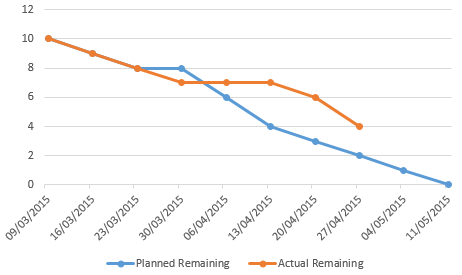
\includegraphics[width=0.8\textwidth]{images/burndown.png}
  \caption{Burndown chart of features implemented and tested fully. X axis represents number of features to implement, whilst Y axis shows the date that the features have been implemented by.}
  \label{fig:burndown}
\end{figure}

Although work appears to be behind schedule here, it should be noted that there is still both time remaining and some features are more than half complete. For strict purposes though and following the FDD manifesto, a feature can not be said to be complete until it is 100\% complete. 

Analysing the graph further, the main problem can be seen where work was halted on feature five, the creation of manoeuvres on the canvas. Becuase issues prolonged work here, it meant other features were pushed back until it was decided that they should be completed in order to make a more whole application. Due to moving onto and completing other features first alongside writing this part of the report, considerable time has been made up. The time remaining will now allow for any completion of features that are most important, and also fixes to others if possible. 

In addition to the graph shown, the features can be expressed as feature sets in the traditional FDD progress report way, by creating

\subsection{After-test fixes and developments}

%fix OLAN, smoke trails too!
%hide movie reel
%fix reel scroll
%parameters OLAN not done
%check if manoeuvres fit

\section{User testing}
Now that the alocated time for implemntation and testing has been used, testing to see how the application meets its initial requirements is important. Along with the JSUnit tests and the usability tetsts that were created, user testing is a means of testing ideal for front-end applications where the usability of the application is paramount. There are a few routes that can be taken to perform user testing, one of which is a questionnaire. Rather than allowing the user to sedn feedback through suggestions or pros and cons, a quicker and more direct way to check the applicatins fulfills its needs is to provide the user with a set of direct questions, allowing them to state if they agree or dissagree. One example could be whether the colour scheme is sutible. By getting the amount agreeing above a certain threshold percentage wise would help show that the colour scheme aspect was correctly applied.

The questionnaire, which can be found in the appendices under appendix D, section~\ref{test:questionnaire} provided ten agree or dissagree questions that the users had to answer. Upon creating the questionnaire, these were then handed to a pick of 10 users, in technical and none-technical backgrounds to ensure a good spread of opinion. If just technical users were chosen, they might not see the application from the aspect of GUI as much as a standard user, as some users may find it harder to find things on a page. Things such as menus for instance may not be as visible and easy to find for users who have not seen similar layouts in the past, and it is important that they application has a level of being self-documenting.

The users selected to perform the testing comprised of eight students and two none-students. It was also ensured that half the students selected were not on a computer science related degree to ensure a wider set of technological knowledge. For each test, a brief description of the application was given to the user explaining the purpose and requiurements of the project and application, followed by the user trying out different features in the GUI and canvas. 

The questionnaires handed out were created using google forms, to keep the process on the internet fo easier tracking. Becuase this form of testing was not planned out originally on the Gantt chart at the start of this project, it was important that the tests were carried out as quickly as possible, so google forms were sent out and asked they could be returned a couple of days later. Indeed all ten questionnaires were returned, each of which all answers had been answered. This was very successful, as it then allowed the results to be analysed properly, and graphs created.

The results of each question can be found in appendix D section~\ref{test:questions}. Looking at the results, it can be assumed that... %TODOOOOOOOOOOOOOOOOOOOOOOOOOOOOO

\section{Implementation and testing review}
On completion of the process of the tests of the final application, a short review of the methods that was used to create the application can now follow. Starting with the pre-coding tasks that had to be completed, Github was intially set up on the machines the applicationw as going to be created on, followed shortly by the set up of Travis and Grunt which was used later for automatic running of tests. Once the repository and branch that would used to host the application was set up, Sublime text was used to perform the coding, and was used becuase of the package compatibilty to assist with code formatting. In terms of how long it took to prepare the enviromnemtn for coding, this took less than a day, including the work blog.

This leads up to time management, where the amount of work done in the implimentation stage was an important factor. Considering that all features had been started and tested by a week before the stage deadline, progress was kept on top of, and it was ensured that tasks that were taking too long did not affect the rest of the application. An example of some of the issues are ones that came from attempting to create the manoeuvres on the canvas with the OLAN interpretations. The first set back was the interpolation issues, which were fixed by changing the curve inclines. Another setback was the issue with cuvres not appearing the go in the correct direction, which was again fixed at the end of the implementation. 

Testing mechanisms used a wide selection of methods, from usability tests to unit tests ensuring that while the back-end methods performed the features as effiecently as possible, the front end allowed users to interact with these features easily. By using the FDD iterative approach, and producing this setion of the report alongside each iteration it has meant that the entire application and documentation has been built in the most stable way.

There are possible improvements that could have been made to this stage of the project though, one such would have been sticking to a much stricter order to features, by creating the base logic to produce the manoeuvres first, rather than getting the GUI up and running. This though would have slowed down testing, so there are weigh-ups both ways.

